\chapter{Projekt systemu}

\section{Przypadki użycia}
	\begin{table}[H]
	\centering
	\sffamily\captionsetup{justification=raggedright,singlelinecheck=false,position = below, font = sf}
	\begin{tabular}{|m{3.5cm}|m{11cm}|}
	\hline 
	UCI & Add Survey \\
	\hline
	Actors & Company \\ 
	\hline
	Preconditions & Company is signed in and is in the dashboard page. \\
	\hline
	Postconditions & Company added survey. \\
	\multirow{6}{*}{Main Success Scenario} & 1.Company hits on 'Add Survey' button. \\
	\cline{2-2}
	& 2.Company hits proper 'Add Question' button depending on what type of question company wants. \\
	\cline{2-2}
	& 3.Company fills up question's content. \\
	\cline{2-2}
	& 4.Company repeats steps from point 2. until completes survey. \\
	\cline{2-2}
	& 5.Company hits 'Add Voucher' button in order to compose survey with concere voucher. \\
	\cline{2-2}
	& 6.Company hits 'Confirm Survey' button. \\
	\hline
	\multirow{4}{*}{Alternate flows} & 2a.Company hits 'Confirm Survey' button without adding any questions: \\
	\cline{2-2}
	& \multicolumn{1}{c|}{1.System signals error and doesn't proceed.} \\
	\cline{2-2}
	& 5a.Company hits 'Confirm Survey' button without adding voucher: \\
	\cline{2-2}
	& \multicolumn{1}{c|}{1.System signals error and doesn't proceed.} \\
	\hline	
	\end{tabular}
	\end{table}		
		
	\begin{table}[H]
	\centering
	\sffamily\captionsetup{justification=raggedright,singlelinecheck=false,position = below, font = sf}
	\begin{tabular}{|m{3.5cm}|m{11cm}|}
	\hline
	UCI & Sign in \\
	\hline
	Actors & Company \\
	\hline
	Preconditions & Company is registered in the System  \\
	\hline
	Postconditions & Company is signed in. \\
	\hline
	\multirow{7}{*}{Main Success Scenario} & 1.Company enters the website and is on landing page \\
    \cline{2-2}
     & 2.Company hits the Sign In button. \\
	\cline{2-2}
     & 3.System moves the Company to the Sign In page.\\
	\cline{2-2}
     & 4.Company enters the login. \\
	\cline{2-2}
     & 5.Company enters the password. \\
	\cline{2-2}
     & 6.Company hits the Sign In/Enter button. \\
	\cline{2-2}
     & 7.System moven the Company to the dashboard page. \\
    \hline
    \multirow{10}{*}{Alternate flows} & 2a.Company hits the Sign Up button: \\
	\cline{2-2}
	& \multicolumn{1}{c|}{1.System moves the Company to the Sign Up page.} \\
	\cline{2-2}
	& 6a.Company hits the Sign Up button or "Doesn't hvae an account? Create one here now!" text. \\
	\cline{2-2}
	& \multicolumn{1}{c|}{1.System moves the Company to the Sign Up page.}	 \\
	\cline{2-2}
	& 6b.Company hits "Forgot the password" text. \\
	\cline{2-2}
	& \multicolumn{1}{c|}{1.Company is guided through password recovery process.} \\
	\cline{2-2}
	& 7a.Invalid login: \\
	\cline{2-2}
	& \multicolumn{1}{c|}{1.System signals error and doesn't proceed/stays on the Sign In page.}	 \\
	\cline{2-2}
	& 7b.Invalid password: \\
	\cline{2-2}
	& \multicolumn{1}{c|}{1.System signals error and doesn't proceed/stays on the Sign In page.} \\
    \hline
	\end{tabular}
	\end{table}
	
	\begin{table}[H]
	\centering
	\sffamily\captionsetup{justification=raggedright,singlelinecheck=false,position = below, font = sf}
	\begin{tabular}{|m{3.5cm}|m{11cm}|}
	\hline 
	UCI & Sign up \\
	\hline
	Actors & Company \\
	\hline
	Preconditions & Company is not already registered in the System. \\
	\hline
	Postconditions & Company is registered in the System. Company is able to access its dashboard. \\	
	\hline
	\multirow{8}{*}{Main Success Scenario} & 1.Company enters the website and is on landing page. \\
	\cline{2-2}
	& 2.Company hits the Sign Up button. \\
	\cline{2-2}
	& 3.System moves the Company to the Sign Up page. \\
	\cline{2-2}
	& 4.Company enters login, password, name and address. \\
	\cline{2-2}
	& 5.Company hits Sign Up/Enter button. \\
	\cline{2-2}
	& 6.System notifies Company about successful registration. \\
	\cline{2-2}
	& 7.System moves Company to the landing page. \\
	\cline{2-2}
	& 8. System can also demand entering a verification token from e-mail after the registration. \\
	\hline
	\multirow{10}{*}{Alternate flows} & 2a.Company hits the Sign In button: \\
	\cline{2-2}
	& \multicolumn{1}{c|}{1.System moves the Company to the Sign In page.} \\
	\cline{2-2}
	& 5a.Company hits Cancel/Back button: \\
	\cline{2-2}
	& \multicolumn{1}{c|}{1.System moves the Company to the landing page.} \\
	\cline{2-2}
	& 6a.Login/e-mail already taken: \\
	\cline{2-2}
	& \multicolumn{1}{c|}{1.System signals error and doesn't proceed.} \\
	\cline{2-2}
	& 6b.Login/Name/Address contains forbidden symbols: \\
	\cline{2-2}
	& \multicolumn{1}{c|}{1.System signals error, suggests the proper symbol range and doesn't proceed.} \\
	\cline{2-2}
	& 6c.Any of registration fields is empty: \\
	\cline{2-2}
	& \multicolumn{1}{c|}{1.System signals error, suggests to fill the empty field and doesn't proceed.} \\
	\hline
	\end{tabular}
	\end{table}
	
	\begin{table}[H]
	\centering
	\sffamily\captionsetup{justification=raggedright,singlelinecheck=false,position = below, font = sf}
	\begin{tabular}{|m{3.5cm}|m{11cm}|}
	\hline 
	UCI & Filling up the survey \\
	\hline
	Actors & User \\ 
	\hline
	Preconditions & None or the mobile app installed required , if user want's to make it that way \\
	\hline
	Postconditions & User accomplished fulfilling the survey. User gain a voucher code. \\
	\multirow{10}{*}{Main Success Scenario} & 1.User chose a company, which voucher might be interesting for him (either in mobile app or website). \\
	\cline{2-2}
	& 2.System moves user to website where the survey is shown. \\
	\cline{2-2}
	& 3.User fulfilss whole survey step by step. \\
	\cline{2-2}
	& 4.User hits 'Done' button. \\
	\cline{2-2}
	& 5.System validates survey and user moves forward. \\
	\cline{2-2}
	& 6.System notifies user that the survey is accepted. \\
	\cline{2-2}
	& 7.System asks user for e-mail Adress	 \\
	\cline{2-2}
	& 8.User can aceppt his e-mail Adress by pressing the button.  \\
	\cline{2-2}
	& 9.System sends voucher to user. \\
	\cline{2-2}
	& 10.System notifies user that the voucher has been sent. \\
	\hline
	\multirow{3}{*}{Alternate flows} & 5a.Survey rejected, validation didn't pass: \\
	\cline{2-2}
	& \multicolumn{1}{c|}{1.Special informations are displayed.} \\
	\cline{2-2}
	& \multicolumn{1}{c|}{2.User is asked to fix his answers.} \\
	\cline{2-2}
	\multirow{3}{*}{Alternate flows} & 9a.User passed e-mail that don't match e-mail address' pattern: \\
	\cline{2-2}
	& \multicolumn{1}{c|}{1.Special informations are displayed.} \\
	\cline{2-2}
	& \multicolumn{1}{c|}{2.User is asked to pass proper e-mail address.} \\
	\hline	
	\end{tabular}
	\end{table}	
	
	
	\begin{table}[H]
	\centering
	\sffamily\captionsetup{justification=raggedright,singlelinecheck=false,position = below, font = sf}
	\begin{tabular}{|m{3.5cm}|m{11cm}|}
	\hline 
	UCI & Add Voucher \\
	\hline
	Actors & Company \\
	\hline
	Preconditions & Company is signed in and is in dashboard page. \\
	\hline
	Postconditions & Company added voucher. \\	
	\hline
	\multirow{5}{*}{Main Success Scenario} & 1.Company hits „Add voucher” button. \\
	\cline{2-2}
	& 2.Company fills up voucher details( some details in plain text,type of discount, discount rate etc.) \\
	\cline{2-2}
	& 3.Company hits „Add voucher” button to add voucher to right survey from dropdown list. \\
	\cline{2-2}
	& 4.Company confirms voucher by „Confirm voucher” button. \\
	\cline{2-2}
	& 5.Voucher is added. \\
	\hline
	\multirow{6}{*}{Alternate flows} & 5a. Voucher already exist: \\
	\cline{2-2}
	& \multicolumn{1}{c|}{1.Proper error message is displayed.} \\
	\cline{2-2}
	& \multicolumn{1}{c|}{2.Filled for is displayed, company is asked to pass diffrent voucher.} \\
	\cline{2-2}
	& 5b.Company didn't pick any survey: \\
	\cline{2-2}
	& \multicolumn{1}{c|}{1.Proper error message is displayed.} \\
	\cline{2-2}
	& \multicolumn{1}{c|}{2.Filled for is displayed, company is asked to pass diffrent voucher.} \\
	\cline{2-2}
	\hline
	\end{tabular}
	\end{table}	
	
	\begin{table}[H]
	\centering
	\sffamily\captionsetup{justification=raggedright,singlelinecheck=false,position = below, font = sf}
	\begin{tabular}{|m{3.5cm}|m{11cm}|}
	\hline 
	UCI & Remove account \\
	\hline
	Actors & Company \\
	\hline
	Preconditions & Company is registered in system. \\
	\hline
	Postconditions & Company doesn’t have an account. \\	
	\hline
	\multirow{5}{*}{Main Success Scenario} & 1.Company hits „Delete account” button \\
	\cline{2-2}
	& 2.Confirmation window appears asking for confirmation. \\
	\cline{2-2}
	& 3.Company confirms the action by entering the password to the site. \\
	\cline{2-2}
	& 4.All information about the company, surveys and coupons are deleted from database. \\
	\cline{2-2}
	& 5.Company sees statement „Your account has been deleted.”. \\
	\hline
	\end{tabular}
\end{table}

\section{Diagramy aktywności}

\begin{figure}[htbp]
  \centering
  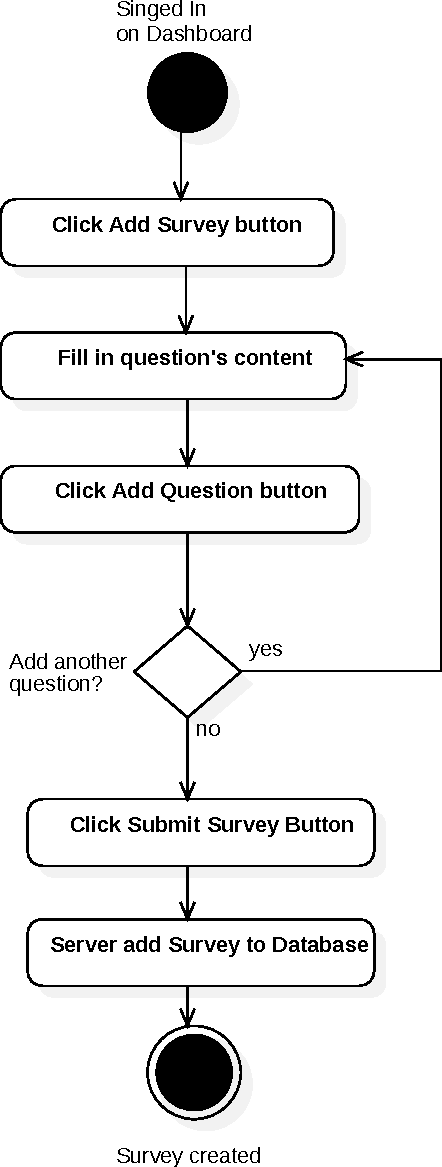
\includegraphics[scale=0.7]{activityCreatingSurvey.pdf}
  \caption{Diagram aktywności dla dodawania ankiety}
\end{figure}
\clearpage

\begin{figure}[htbp]
  \centering
  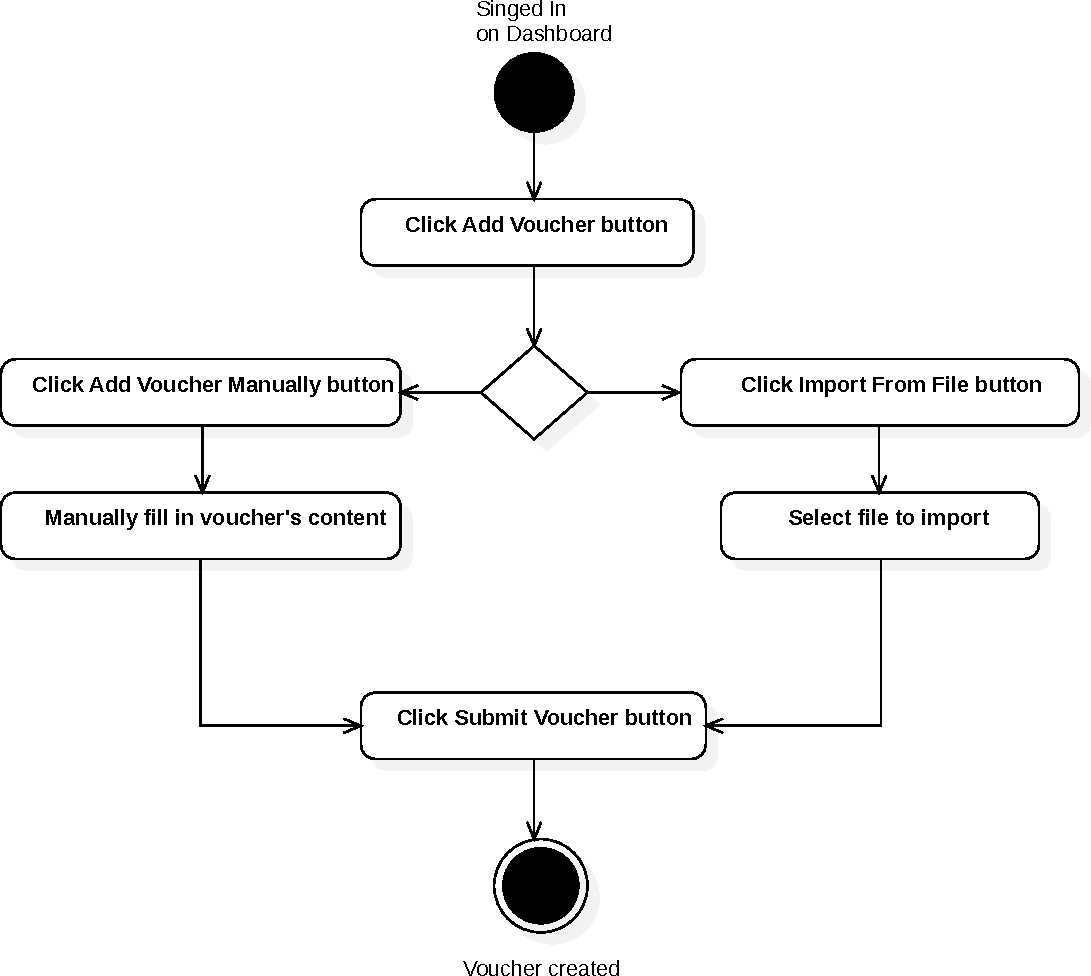
\includegraphics[scale=0.7]{ActivityDiagramCreatingVoucher.pdf}
  \caption{Diagram aktywności dla tworzenia vouchera}
\end{figure}
\clearpage

\begin{figure}[htbp]
  \centering
  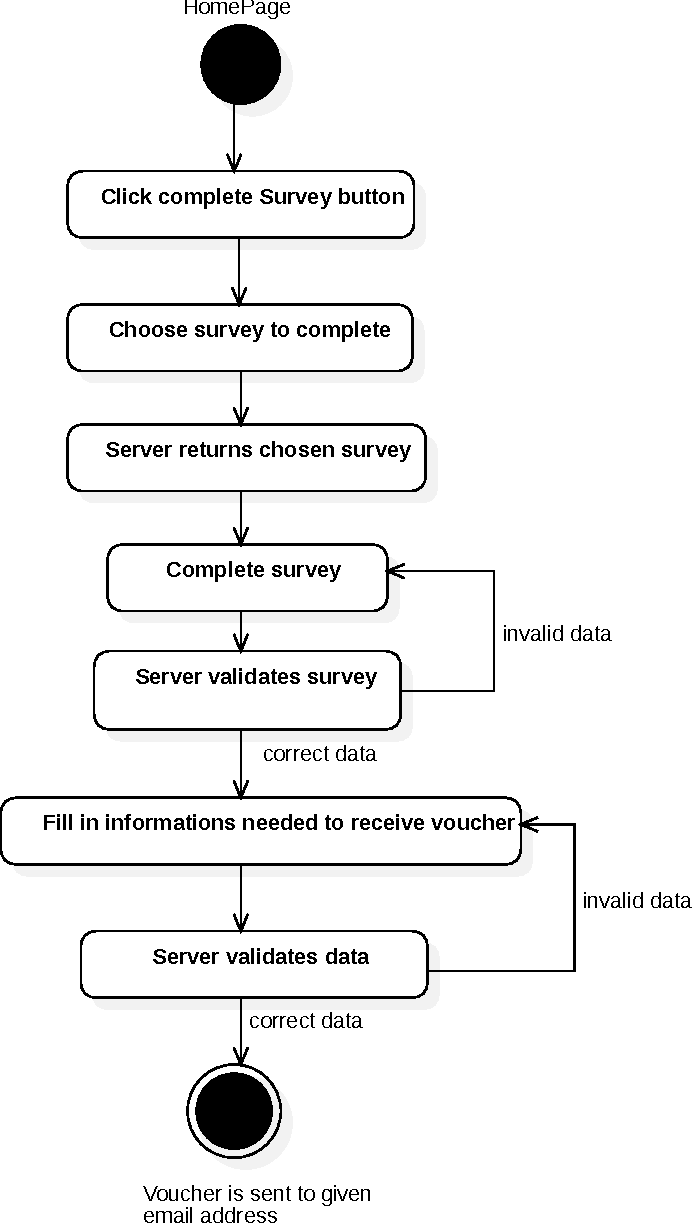
\includegraphics[scale=0.7]{ActivityDiagramGettingVoucher.pdf}
  \caption{Diagram aktywności dla otrzymywania vouchera}
\end{figure}
\clearpage


\begin{figure}[htbp]
  \centering
  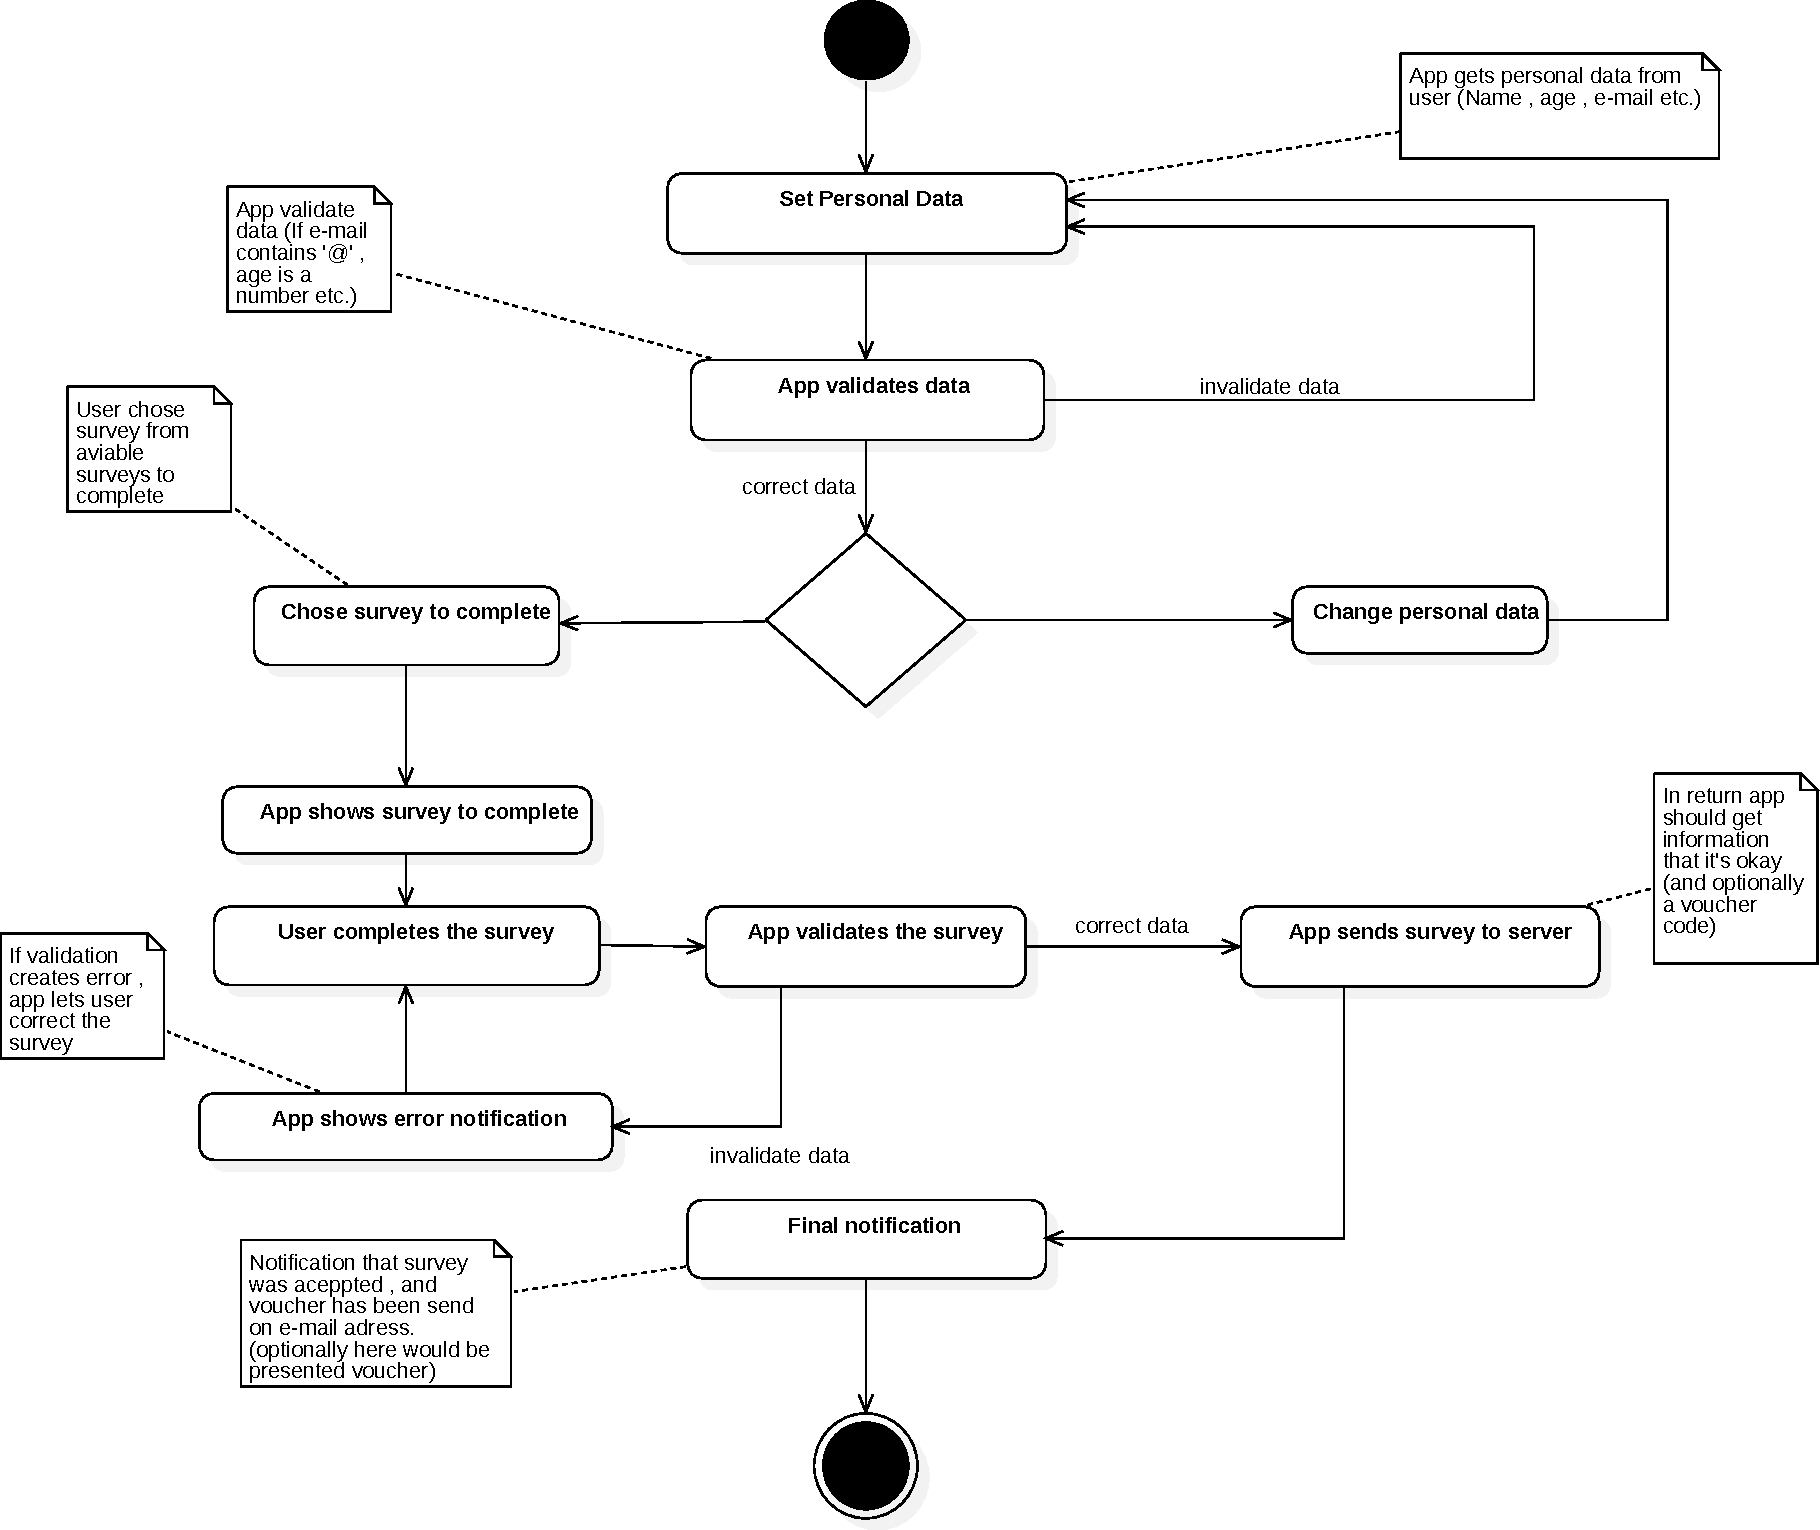
\includegraphics[scale=0.5]{MobileAppActivityDiagram.pdf}
  \caption{Diagram aktywności dla aplikacji mobilnej}
\end{figure}

\begin{figure}[htbp]
  \centering
  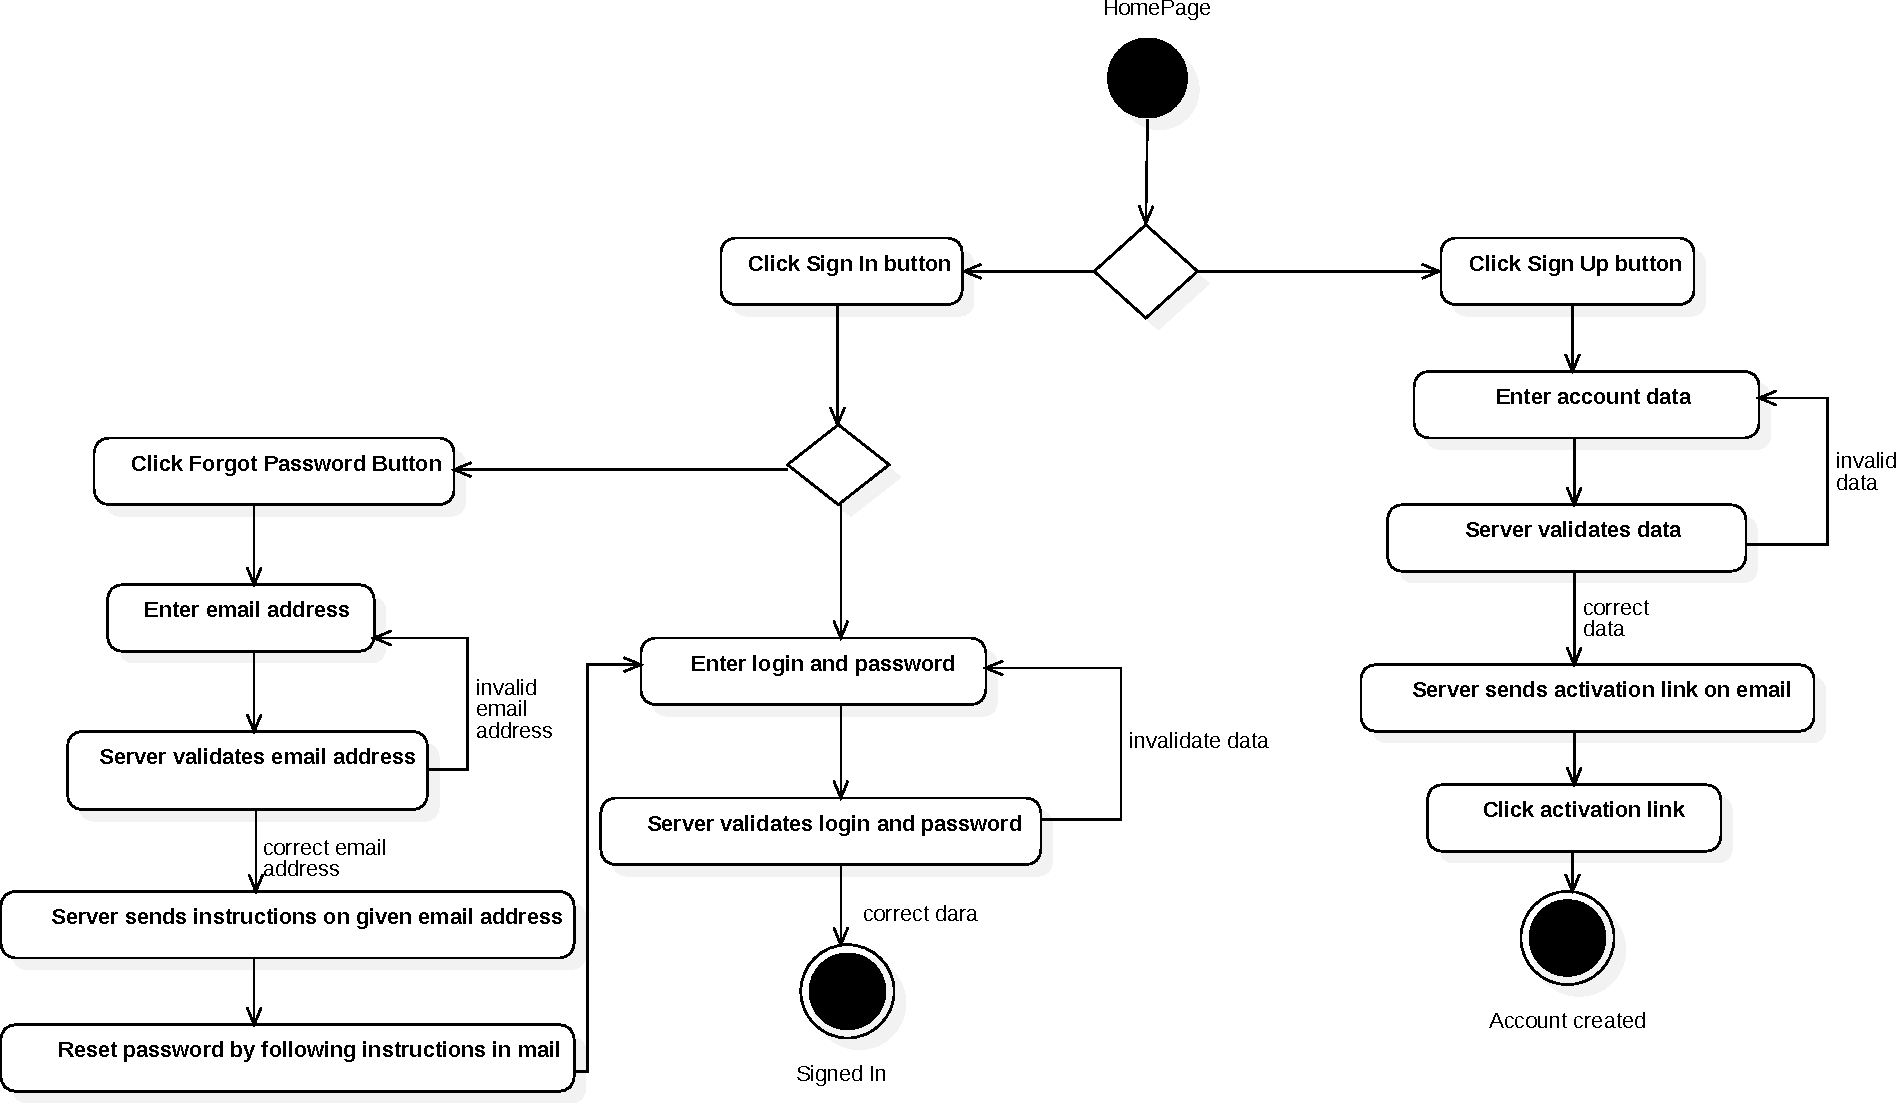
\includegraphics[scale=0.5]{activitySISU.pdf}
  \caption{Diagram aktywności dla logowania i rejestracji}
\end{figure}

\section{Diagramy klas}

\begin{figure}[htbp]
  \centering
  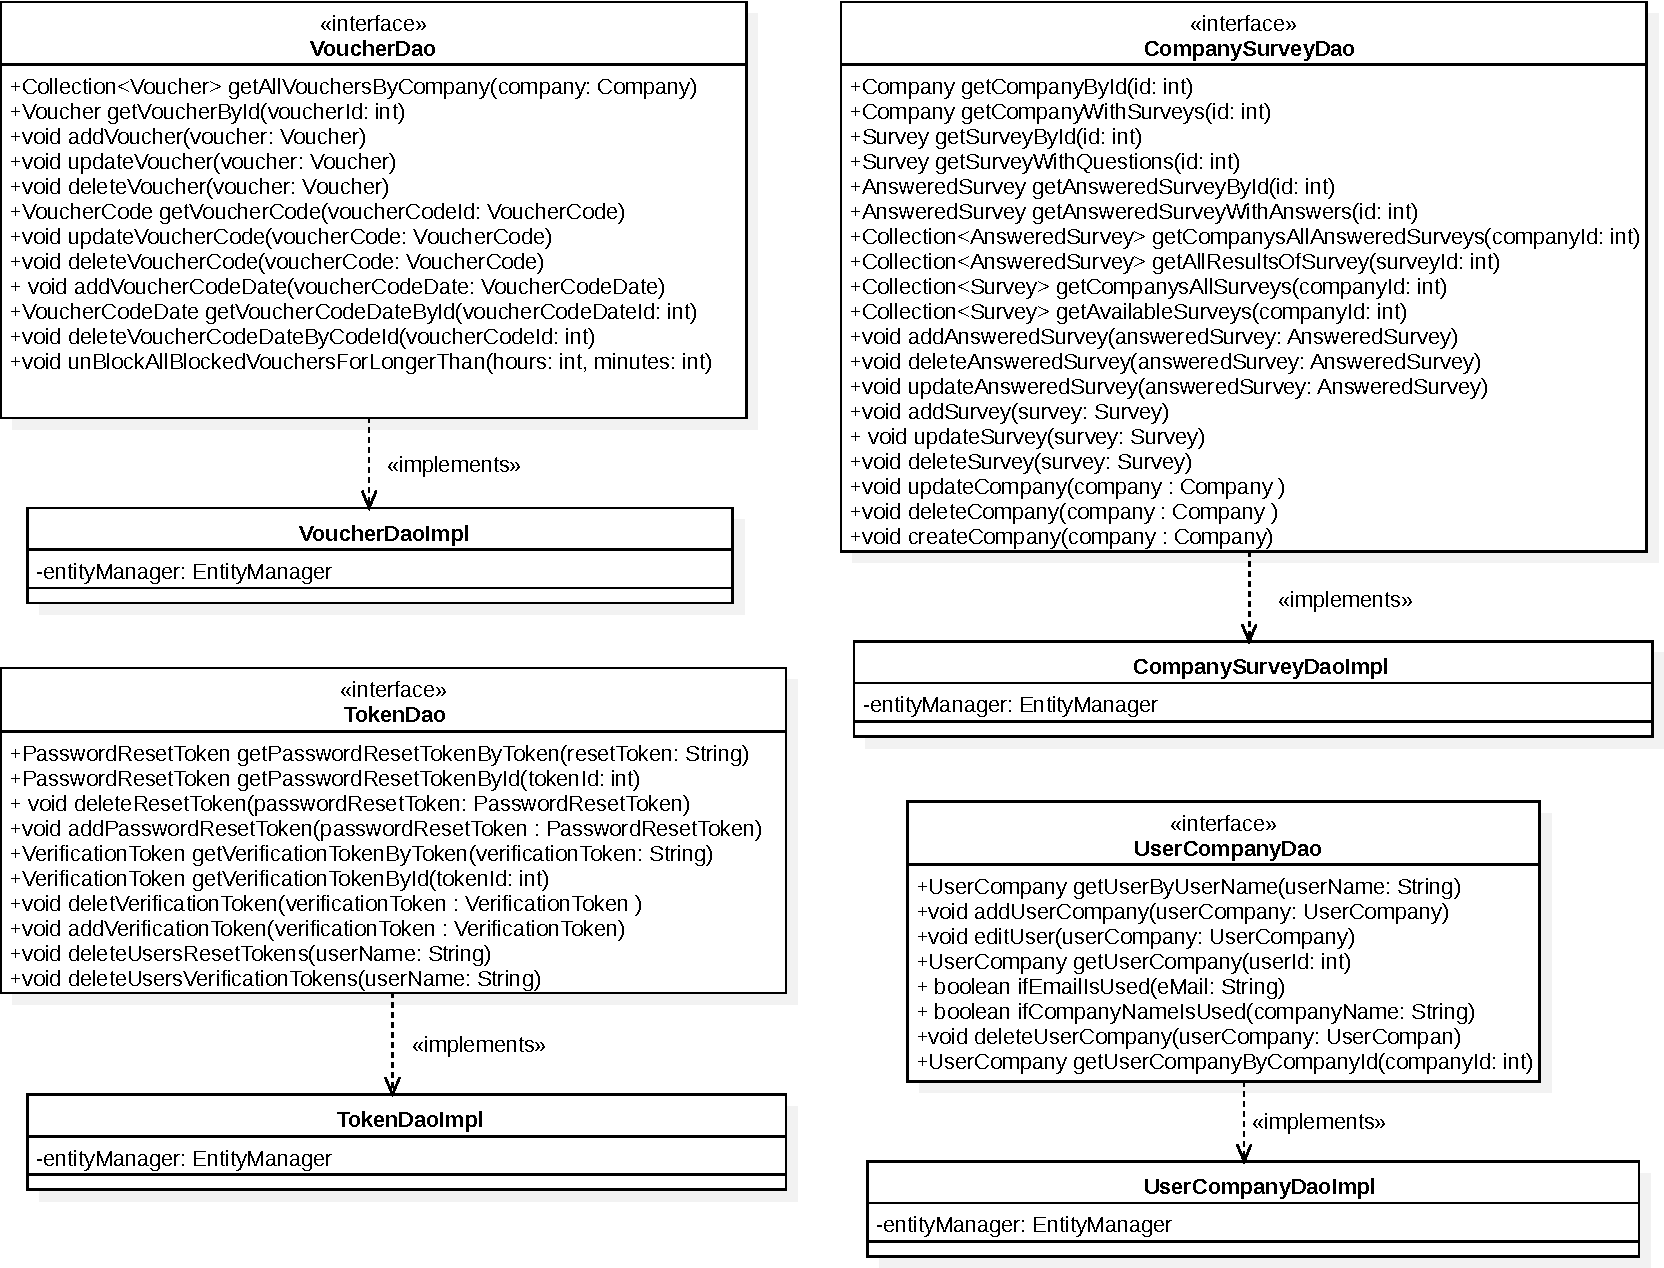
\includegraphics[scale=0.5]{daoUML.pdf}
  \caption{Diagram klas dla DAO}
\end{figure}

\begin{figure}[htbp]
  \centering
  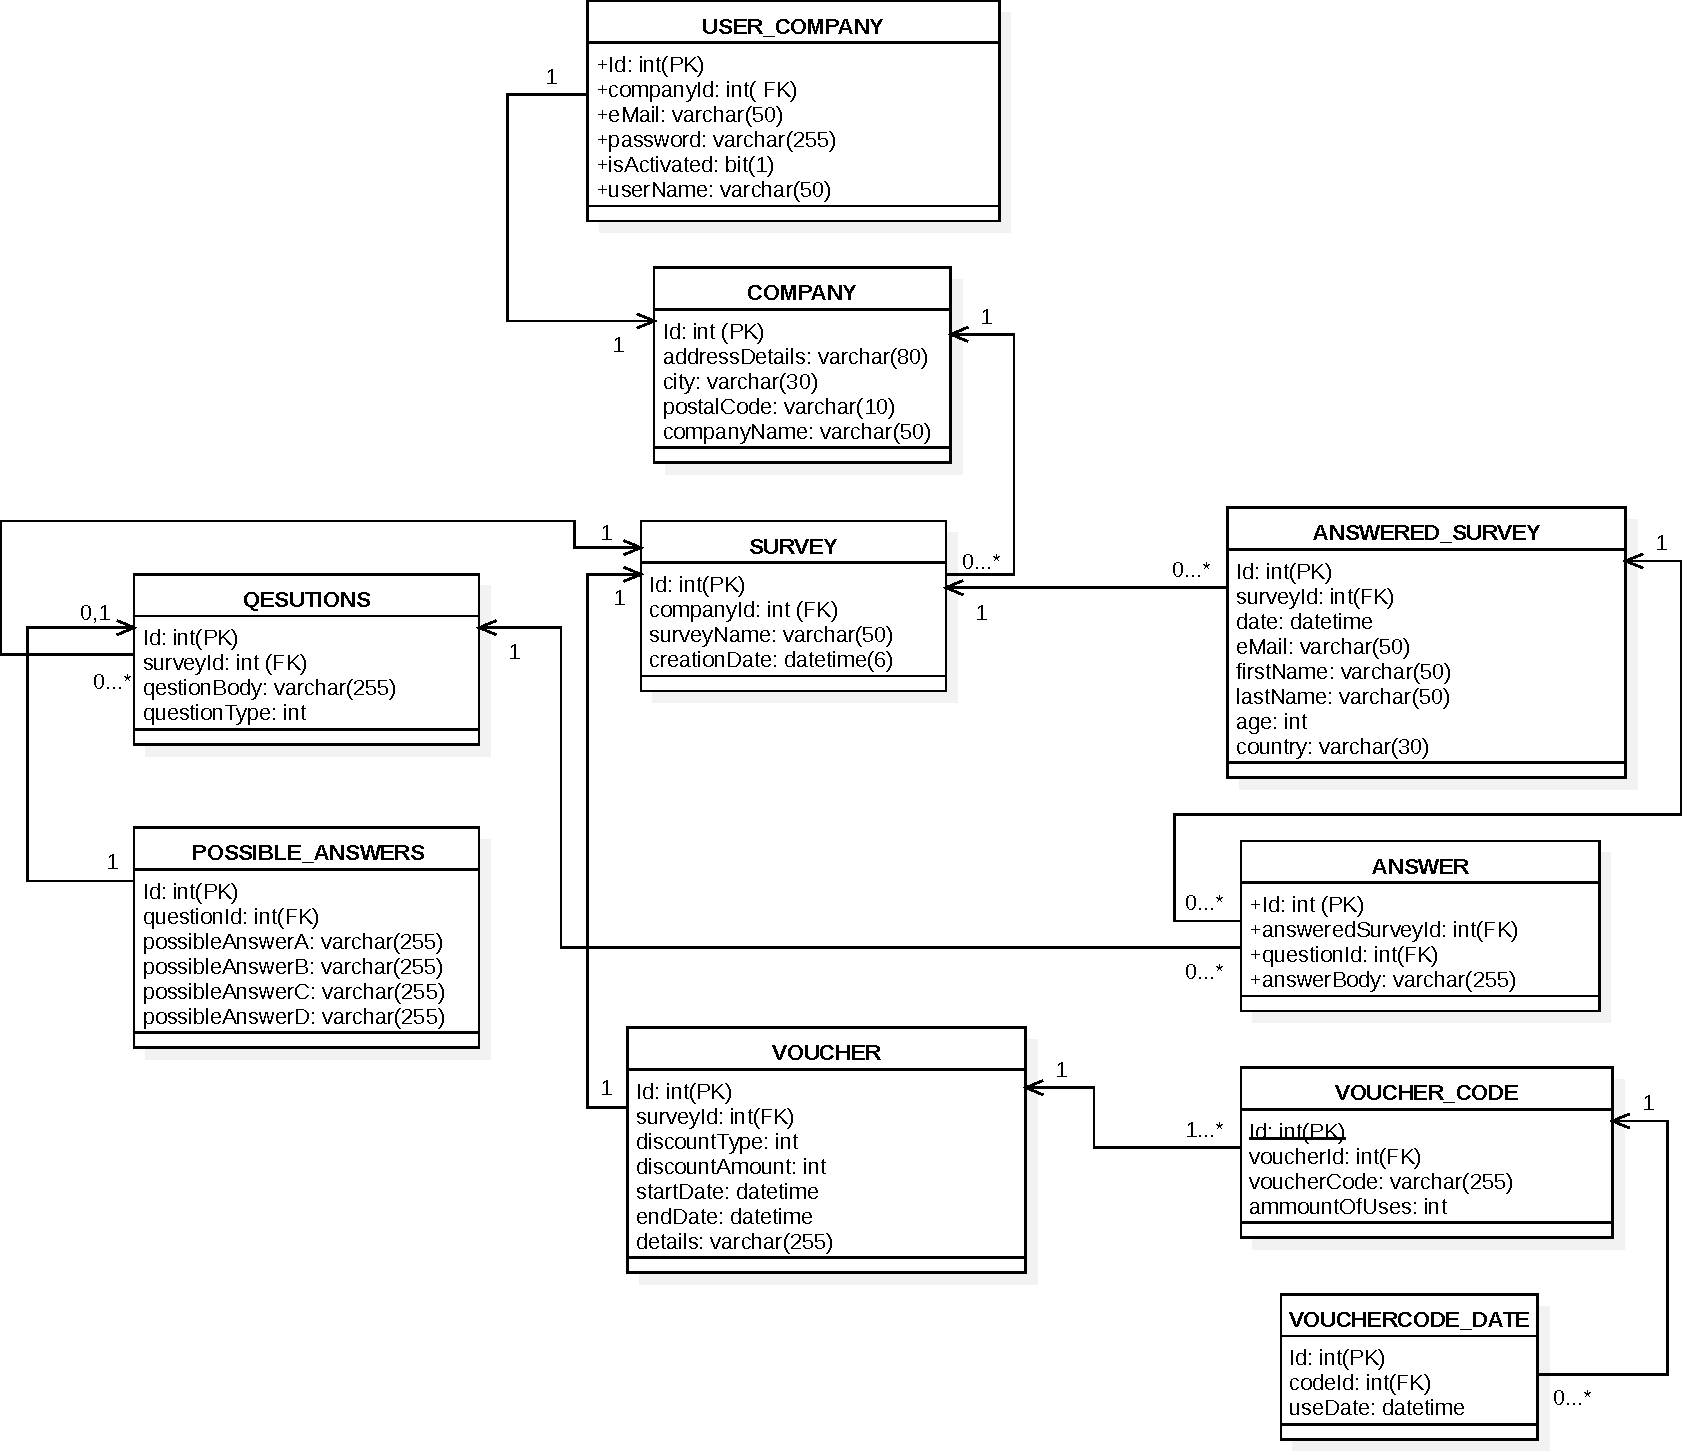
\includegraphics[scale=0.5]{dbUML.pdf}
  \caption{Diagram klas dla bazy danych}
\end{figure}

\begin{figure}[htbp]
  \centering
  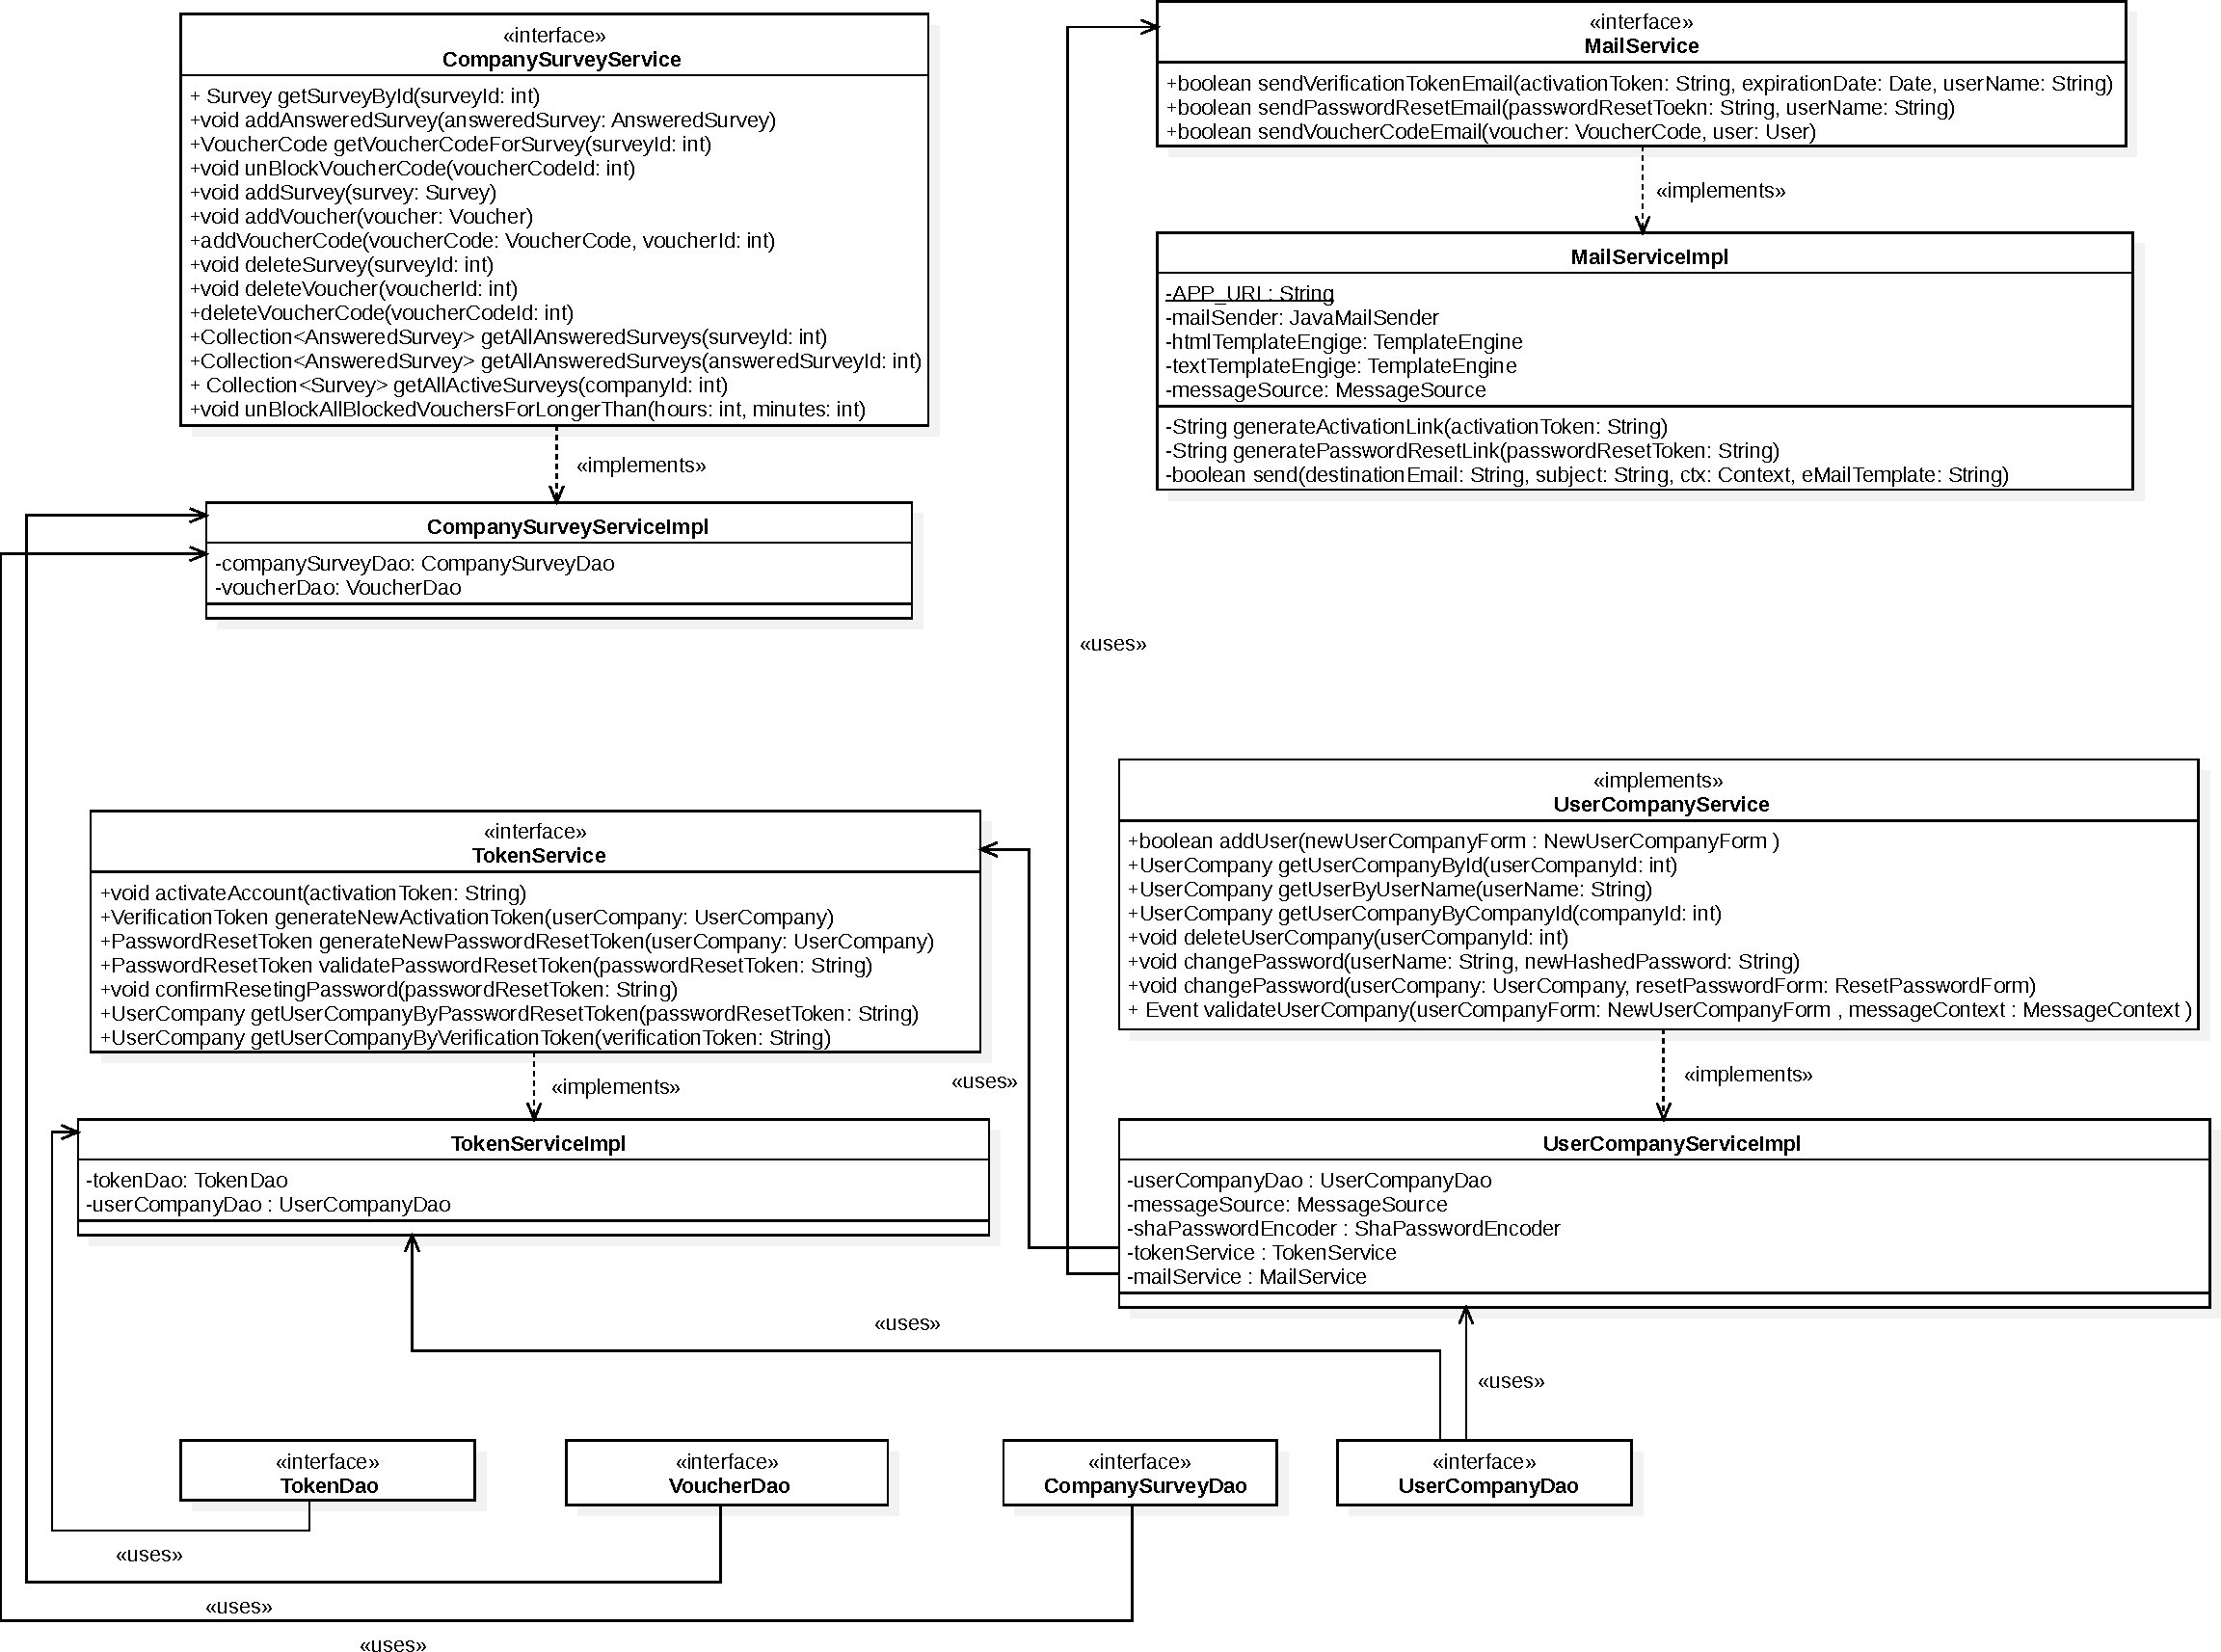
\includegraphics[scale=0.4]{servicesUML.pdf}
  \caption{Diagram klas dla serwisów}
\end{figure}

\section{Diagramy sekwencji}

\begin{figure}[htbp]
  \centering
  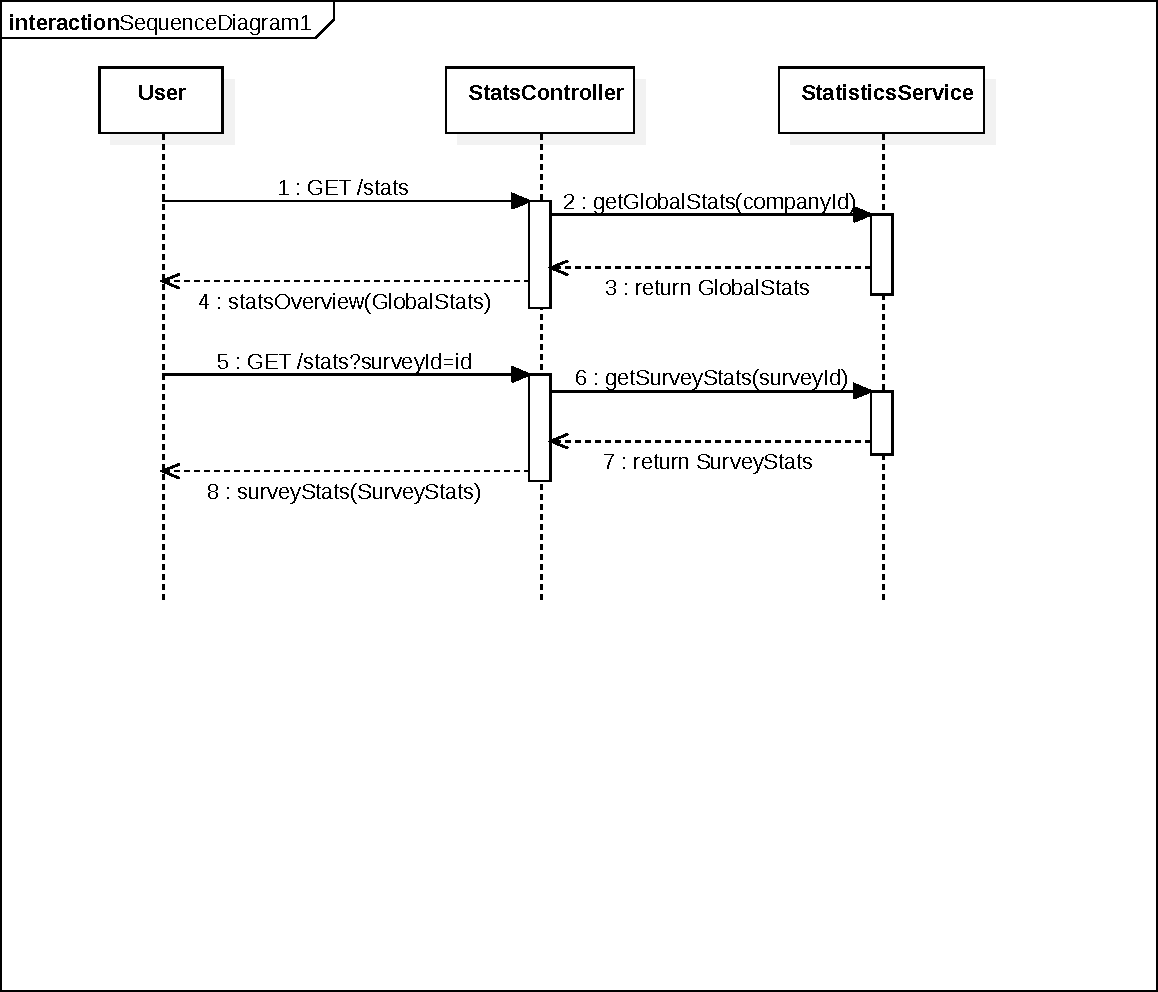
\includegraphics[scale=0.7]{SequenceUMLgetStats.pdf}
  \caption{Diagram sekwencji dla statystyk}
\end{figure}


\begin{figure}[htbp]
  \centering
  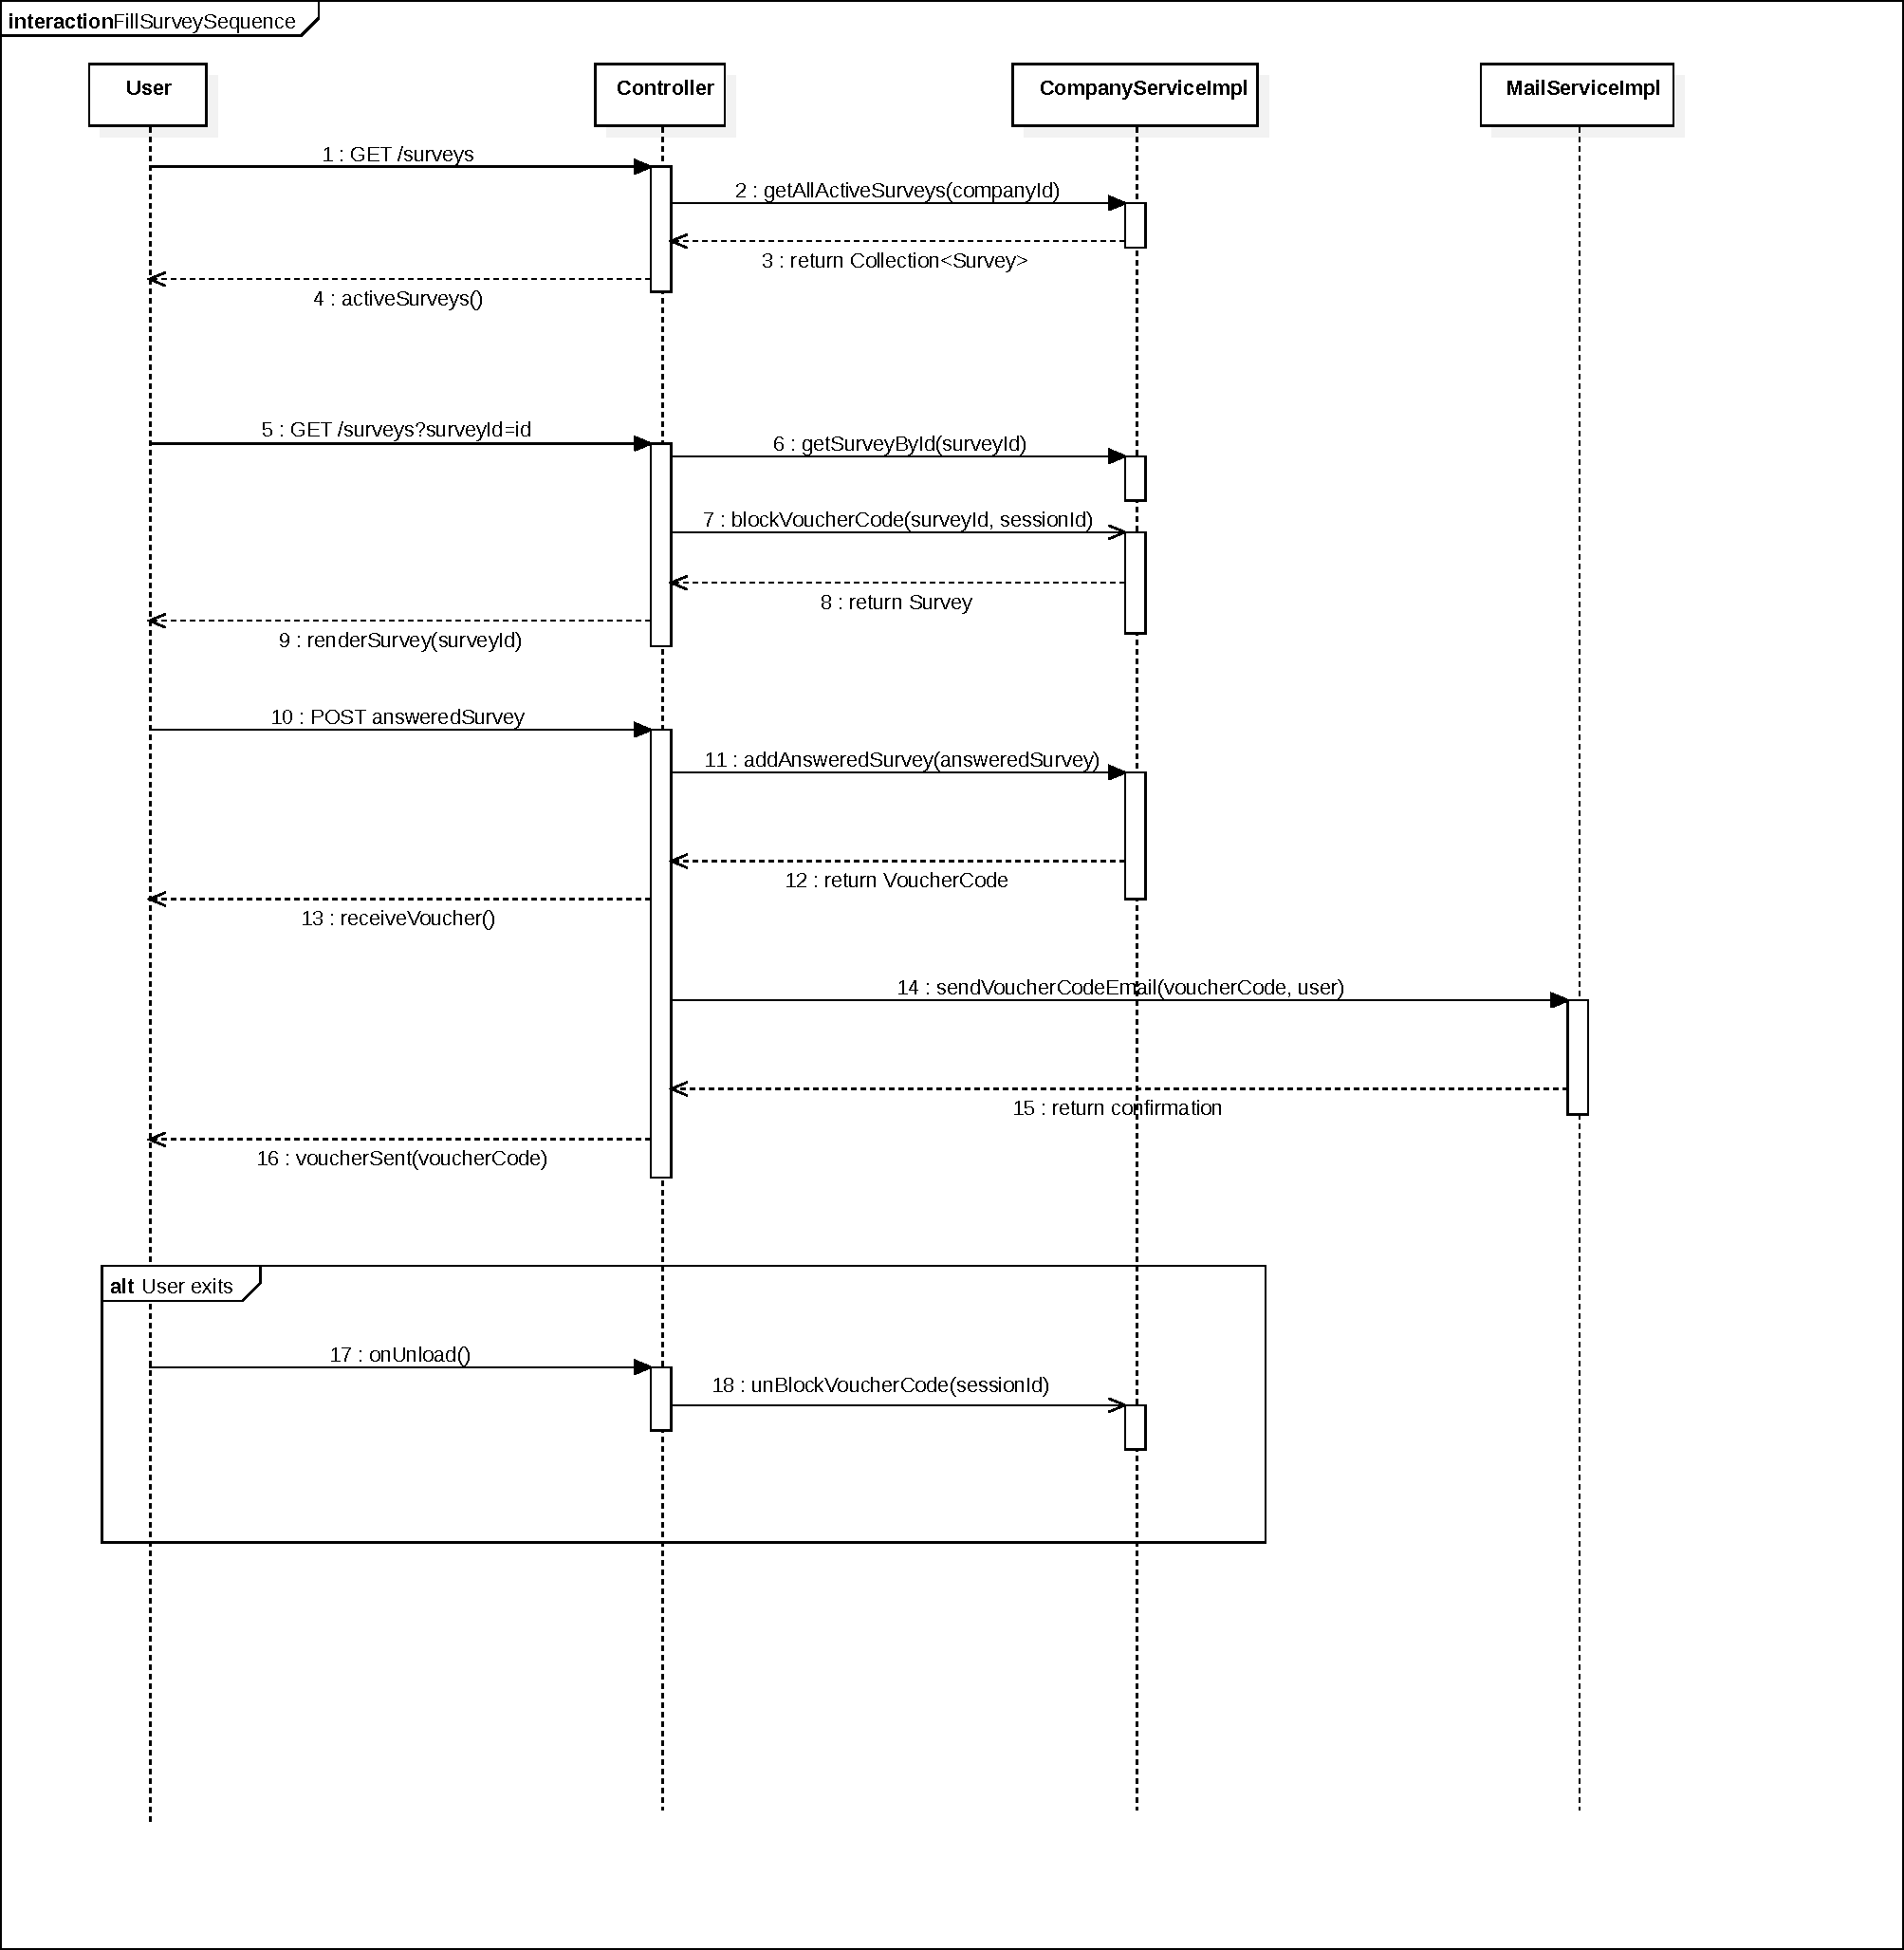
\includegraphics[scale=0.5]{SequenceUMLFillSurvey.pdf}
  \caption{Diagram sekwencji dla wypełniania ankiety}
\end{figure}
